\subsection{Evaluation of Classification of Tweets}
Evaluation is one of the most important part of a categorization process, but it is also one of the most difficult processes. This part is therefore very interesting for our project when deciding how to evaluate our own results. The evaluation process chosen has to be able to decide how whell the classification behaves.
%that the classificaton behaves as desired. 


%has to be chosen so that the results from the process tell if the cal


%Evaluation is one of the most important part of a categorization process because it tells if the classification behaves as desired. Classification is, as already mentioned, difficult to evaluate and it was therefore quite useful to look at the evaluation part of the classification of tweets.

The authors of \emph{Classification of Tweets} argued that the automatic classification should be compared by manual classification i.e., classification done by humans. The results from the automatic classification is marked as \emph{predicted results} and the results from the manual classification is marked as \emph{correct results}. This comparison would give the best indication of the correctness of the classification, but the problem is performing such a comparison on the whole classification which is not possible. Instead, they chose a samle of 500 tweets, where 477 of these were chosen for evaluation of the classification process. All of these were given tags by people, and then the tags were compared to the tags distributed by the classification process. 


%classification done by humans, so that the \textit{predicted} result could be compared with the \textit{correct} result. The problem is that it is very time consuming for humans to classify, so the evaluation was done by sampling 500 tweets. Of these tweets were 477 manually identified by people to give them tags which were compared by the classifier's tags. 
\begin{figure}[H]
\centering
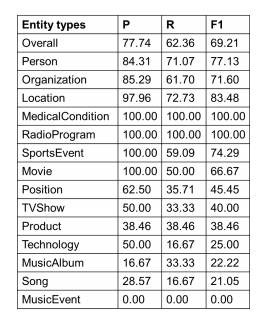
\includegraphics[width=0.5\textwidth]{Chapters/PreviousWork/Classification_entities}
\caption[The accuracy of the system for extraction and linking]{The accuracy of the system for extraction and linking, where \emph{P} is the precision, \emph{R} is the recall and \emph{$F_{1}$} is the \emph{$F_{1}$}-score.}
%P is the precision, R is the recall and $F_{1}$ is the $F_{1}$-score.} %linking\footnote{\url{http://pages.cs.wisc.edu/~anhai/papers/doctagger-vldb13.pdf, page 8}}}
\label{fig:classification_entities}
\end{figure}


Figure \ref{fig:classification_entities} shows the results of the evaluation phase of the classification. The \emph{Classification of Tweets} chose to use 3 common measures for the accuracy of the classification. 
\begin{itemize}
\item[-] \emph{P} (\emph{precision}): fraction of tagged tweets that were relevant. 
\item[-] \emph{R} (\emph{recall}): fraction of relevant tweets that were tagged. 
\item[-] \emph{$F_{1}$-score} (\emph{accuracy}): how accurate the overall results are, defined as:

\[F_1 = 2 \cdot \frac{\mathrm{precision} \cdot \mathrm{recall}}{\mathrm{precision} + \mathrm{recall}}\]
\end{itemize}
The results from figure \ref{fig:classification_entities} are relevant in our project as well, since they give a good indication on which subjects the classifier found difficult to classify. The figure shows that people and locations are easy to classify, while music is more difficult. This could be because music might contain common words that are dropped from the knowledge base or does not provide useful information while name of locations are easy to recognize for the classifier. 

%These observations could be used in our implementation?


%It is interesting to look at the results from the evaluation because they give a good indication on which subjects are difficult to classify. The results show that people and locations are easy to classify, while music is more difficult. This could be because music might contain common words that are dropped from the knowledge base or does not provide useful information while name of locations are easy to recognize for the classifier. 
%One of the most important steps of classifying is the evaluation phase. Evaluation of classifying should be done by humans. Someone will have to look through the results and see how well the classification has been done by comparing the \textit{correct} result with the \textit{predicted} result.

%The article concludes that the tweets that were easiest to classify were about people (see Figure \ref{fig:classification_entities}). This is probably because famous people have their own Wikipedia page, which is easy to match the tweet. The most difficult, on the other hand, was products which seldom have their own page  if the tweet is very specific. 



%Some of these results were worth noting for our proje. 

% Disse resultatene er relevante for oss og for videre arbeid. Kanskje kan man vekte ned der det virker som et er vanskelig. 